% Anhänge, beliebig, kein Zwang
\chapter{Anhang}

% \colorbox{orange}{Datenblätter, Listen, Bedienungsanleitungen, Controller, im Text vorne drauf hinweisen, gleiche Messungen in den Anhang, Ergebnisse vorne}




%\clearpage

\section{Beurteilung von Lastenhandhabungen anhand von Leitmerkmalen}\label{cha_Anhang_5}

\clearpage

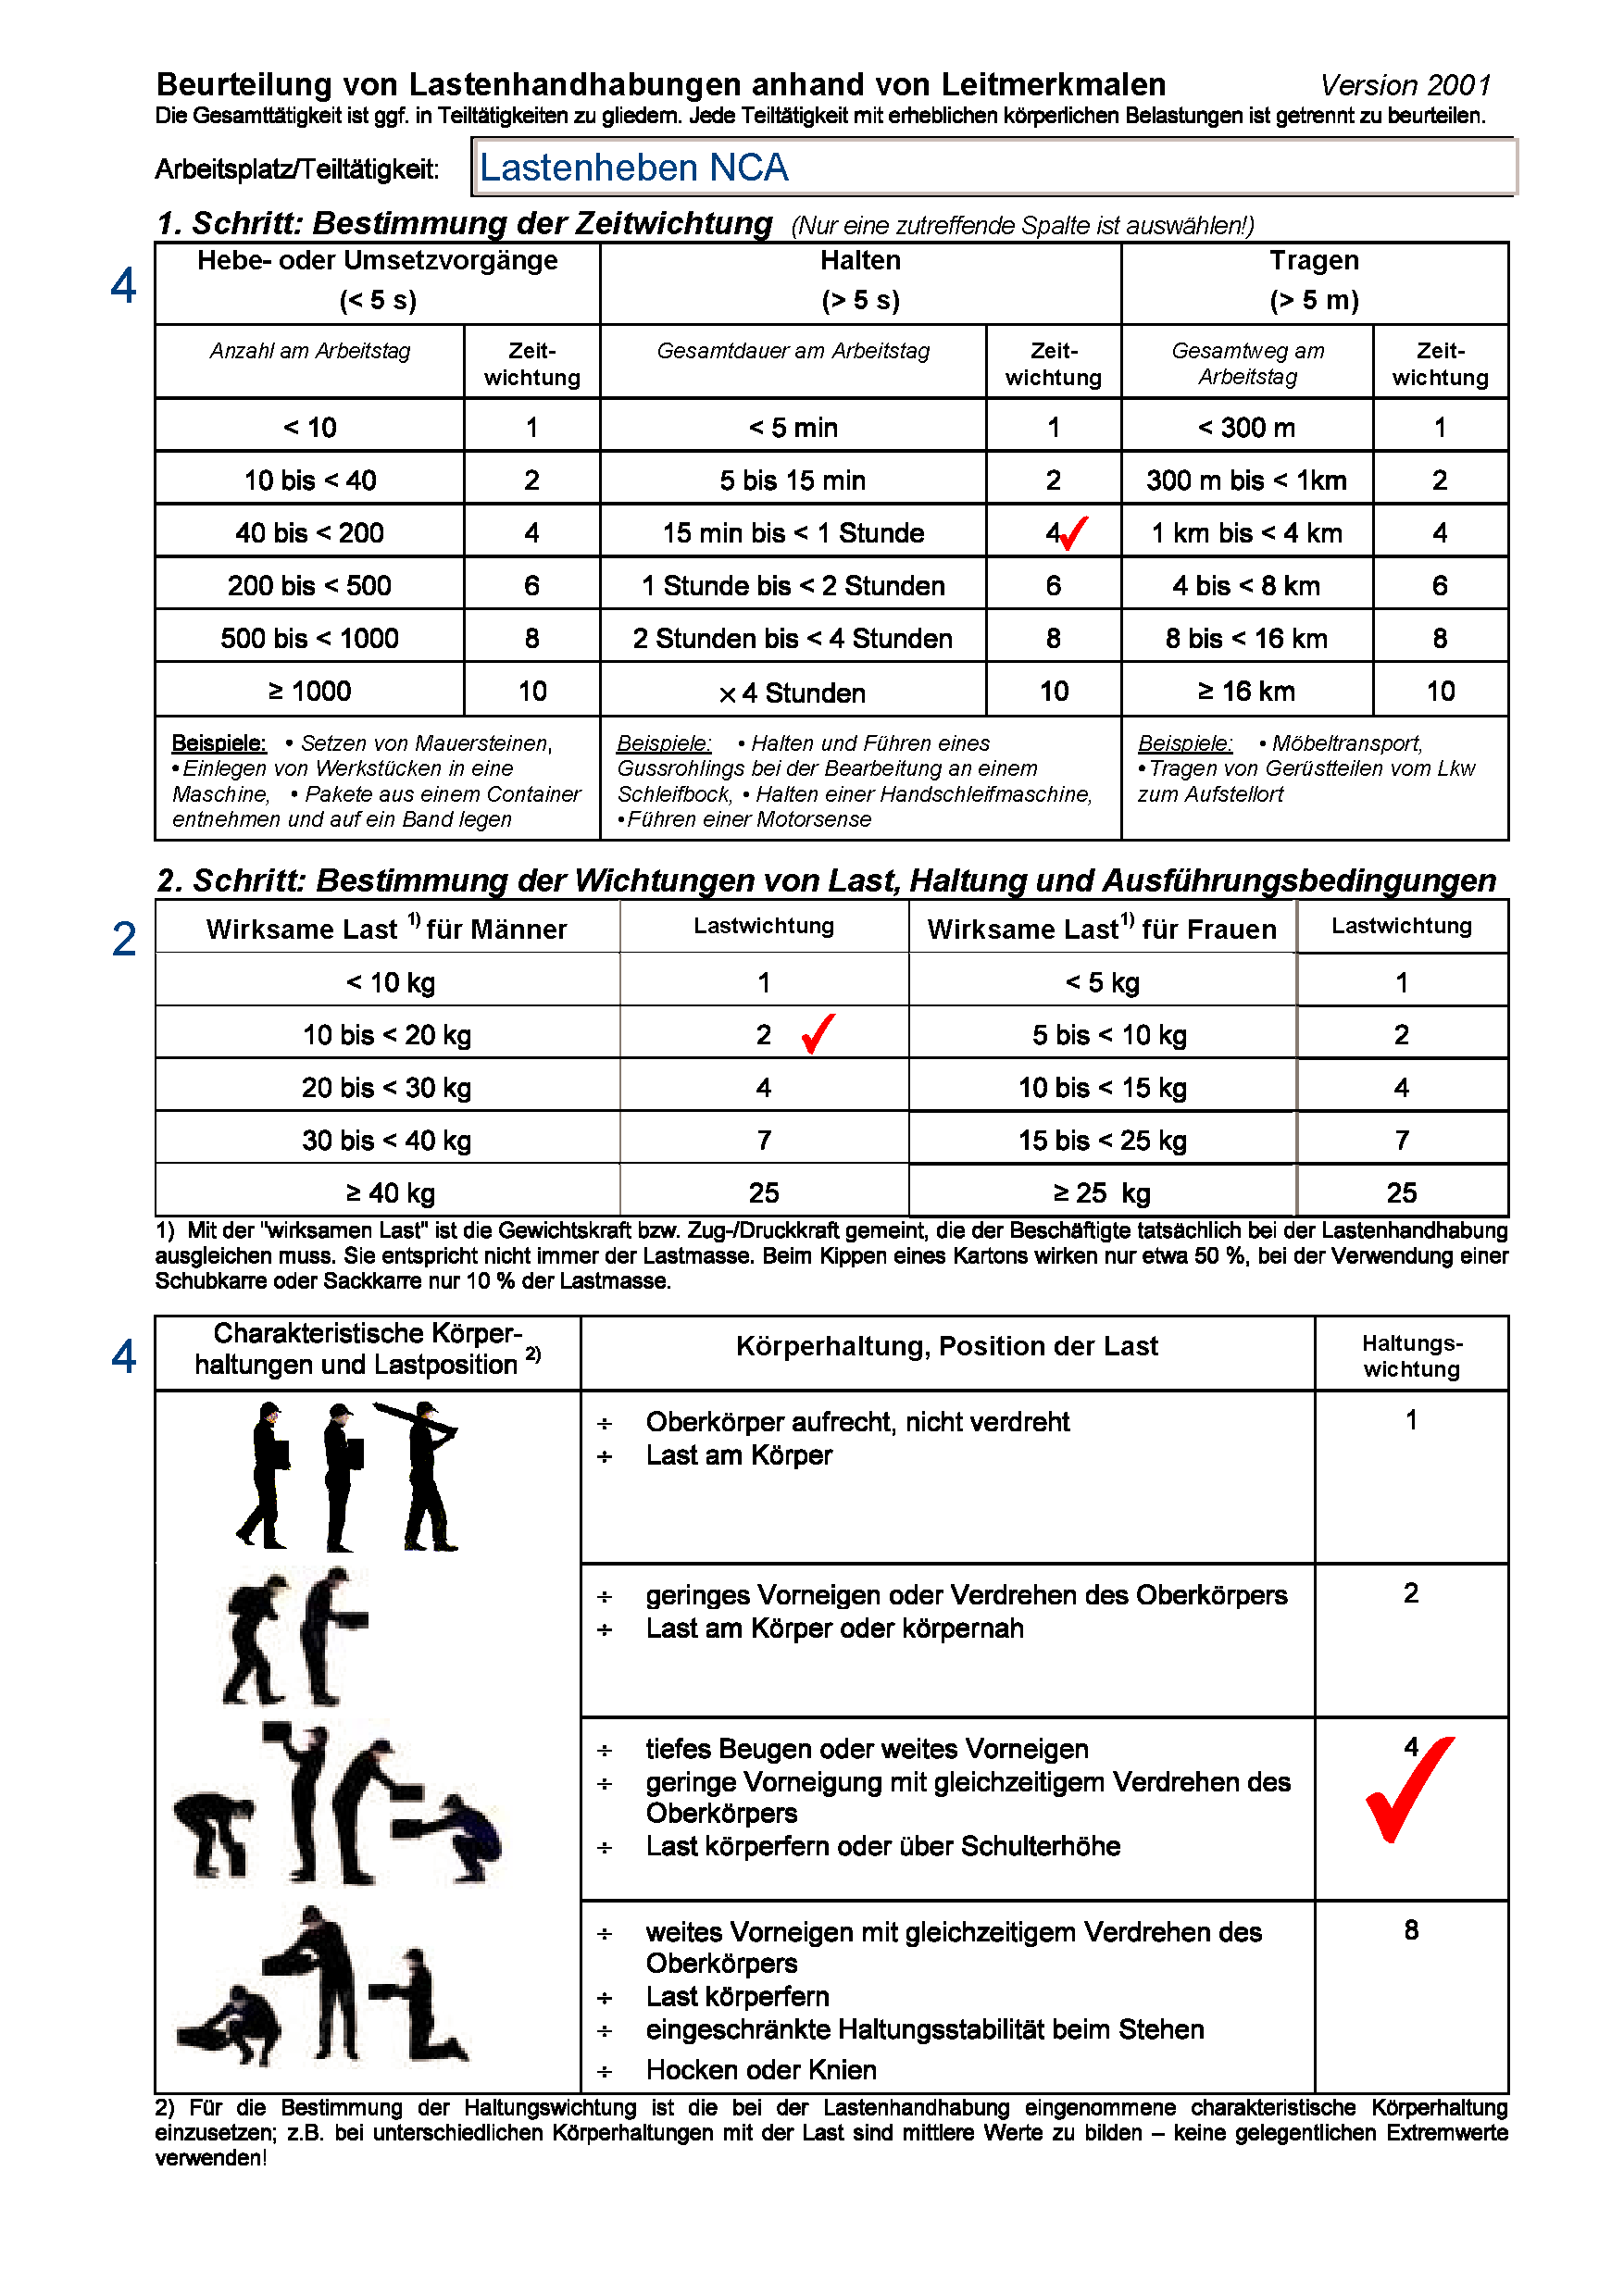
\includegraphics[page=1,width=\textwidth]{anhang/LMM-Heben-Halten-Tragen.pdf}

\clearpage

\includegraphics[page=2,width=\textwidth]{anhang/LMM-Heben-Halten-Tragen.pdf}


\section{Überblick über NC-Aggregate}\label{cha_Anhang_4}



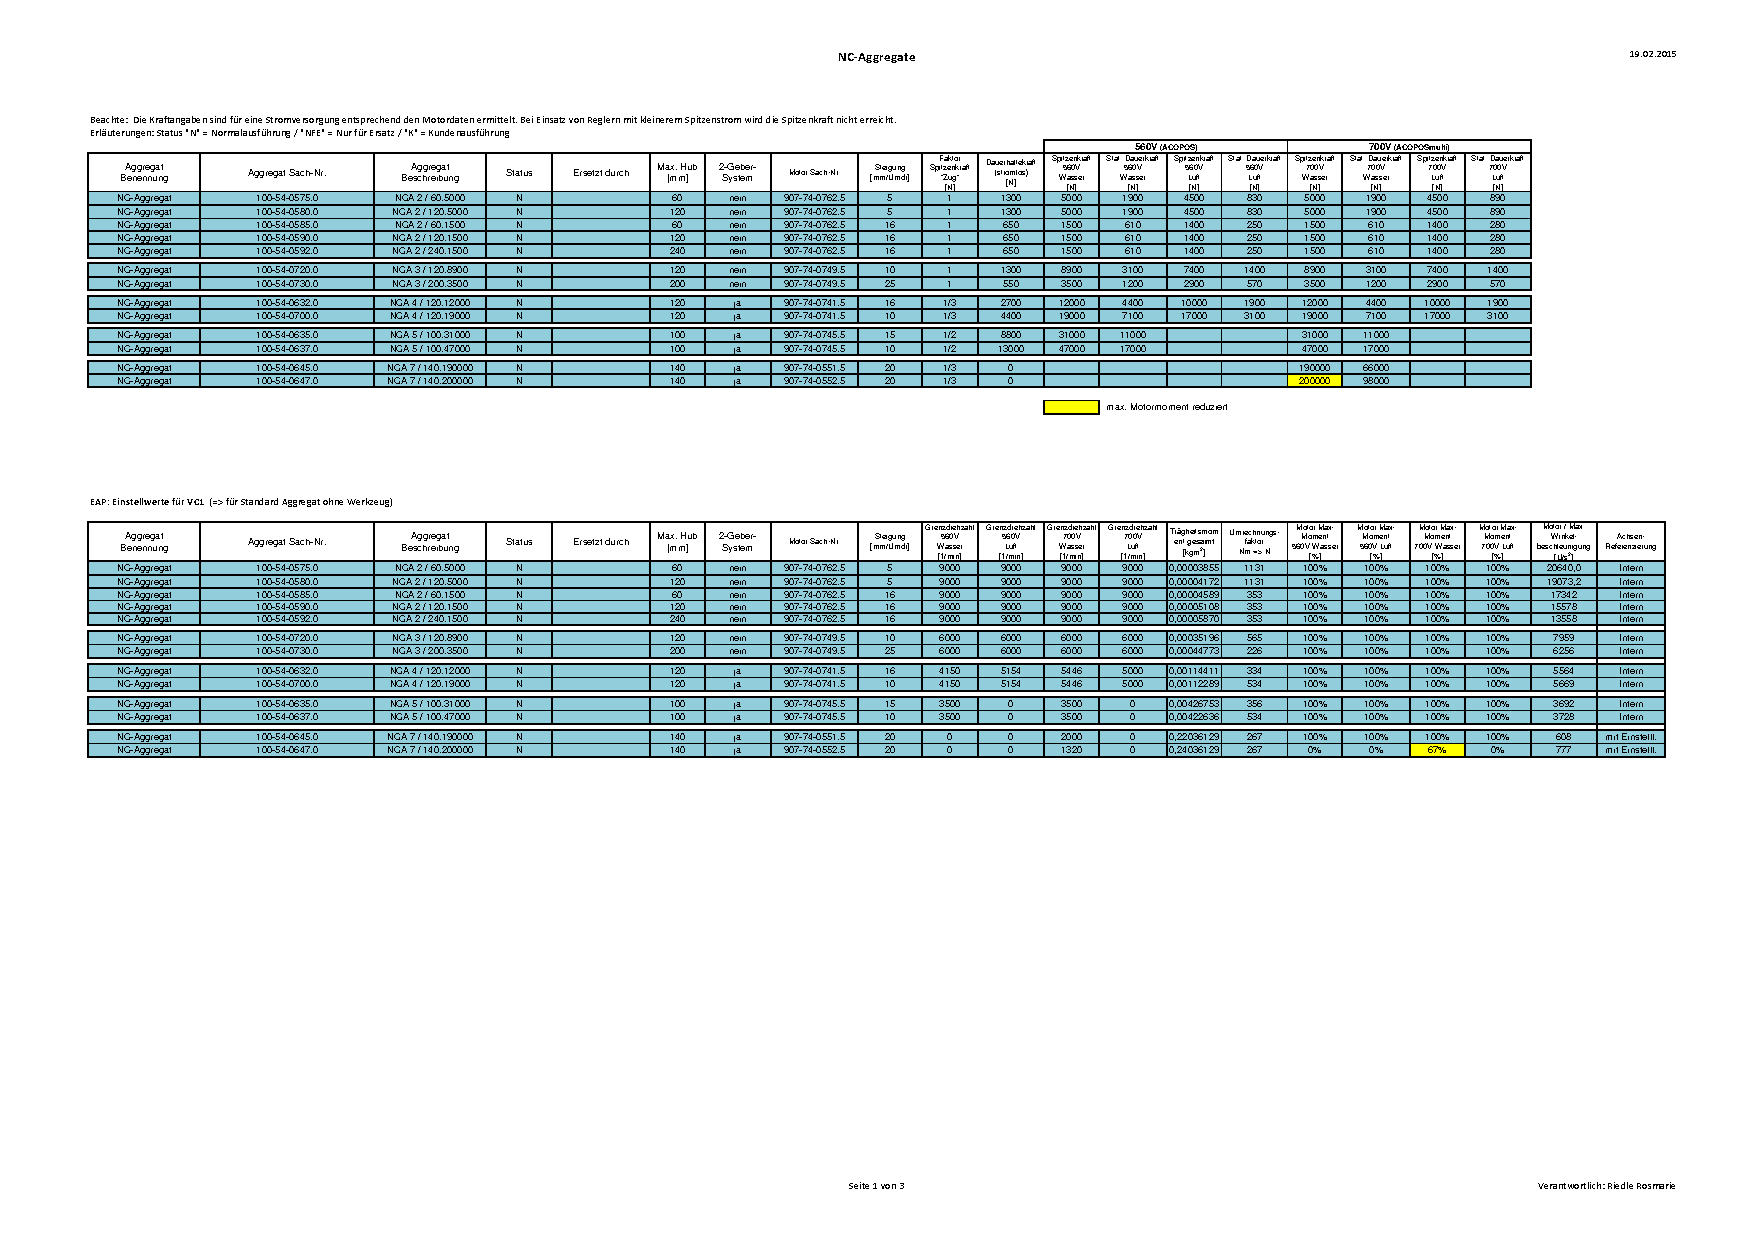
\includegraphics[page=1,angle=90,width=\textwidth]{anhang/Ueberblick_Ueber_NC_Aggregate.pdf}

\clearpage

\includegraphics[page=2,angle=270,width=\textwidth]{anhang/Ueberblick_Ueber_NC_Aggregate.pdf}

\clearpage

\includegraphics[page=3,angle=90,width=\textwidth]{anhang/Ueberblick_Ueber_NC_Aggregate.pdf}


\clearpage




\section{Übersicht über aufgetretene Fehler}\label{cha:Uebersicht_ueber_aufgetretene_Fehler}




\begin{itemize}
 \item konstruktive Fehler
 \begin{itemize}
    \item Kleber für Messlineal ist nicht für die ölhaltige Umgebung und Temperaturen vorgesehen
    \item Der konstruktive Fehler, dass Schmieröl in den Motor und anschließend in den Motorgeber gelangen kann, wurde bereits durch konstruktive Maßnahmen beseitigt. Allerdings sind noch einige Achsen mit dieser Schwachstelle im Umlauf. So ist in der nächsten Zeit mit weiteren Reklamationen aufgrund dieser Ursache zu rechnen.
 \end{itemize}
 
 
 
 
 
 \item Fertigungsfehler der Einzelkomponenten
 \begin{itemize}
    \item Immer wieder müssen nicht zeichnungsgemäß gefertigte Bauteile nachgearbeitet oder ausgetauscht werden. Dies führt zu erheblichen Verzögerungen während der Montage.
 \end{itemize}
 
 
 
 \item Fehler bei der Montage 
 \begin{itemize}
    \item Durch Fehler bei der Montage ergibt sich axiales Spiel, insbesondere durch nicht richtiges Anziehen der Spannmutter in der Pinole. Durch abändern der Montage Reihenfolge kann das falsche Anziehen der Spannmutter verhindert werden. Durch falsches Abstimmen der Abstimmscheibe kann es allerdings immer noch zu axialem Spiel kommen.
    \item Durch nicht richtig abgestimmte Abstimmscheiben kann es entweder zu axialem Spiel oder einer zu großen Vorspannung der Lager kommen.
 \end{itemize}
 
 
 
 
 \item fehlerhafte Programmierung
 \begin{itemize}
    \item Falsch programmierte Parameter treten immer wieder auf, da beim Einrichten eines neuen Werkzeuges alle Parameter für das Aggregat manuell eingegeben werden müssen. Dies führt immer wieder zu unerwarteten Fehlern und längeren Fehlersuchen.
 \end{itemize}
 
 
 \item nicht bestimmungsgemäßer Gebrauch
 \begin{itemize}
    \item Überlastung des Motors. Reklamation
    \item Gleitstein beschädigt (auf Block gefahren). Falsche Handhabung oder falsche Programmierung
 \end{itemize}
 
 
 
 
 \item nicht bestimmungsgemäße Instandhaltung
 \begin{itemize}
    \item Kühlkreislauf ist zugesetzt. Dies ist insbesondere ein Problem bei unsachgemäßen Umgang mit dem Kühlschmiermittel. Auch durch Späne oder sonstige Gegenstände in den Kühlkanälen ist der Durchfluss nicht sichergestellt.
 \end{itemize}
 
 
 \item Verschleiß und Alterungserscheinungen
 
 \clearpage
 
 \item nicht eindeutig zuordenbare Fehler
 \begin{itemize}
    \item Fressen bzw. vorher Verkratzen der Laufflächen der Pinole. Eine mögliche Ursache ist hier mangelnde Schmierung. Es ist bekannt, dass eine außermittige Belastung dieses Problem verschärft, genauso wie sehr kurze Verfahrbewegungen. so dass nicht der ganze Weg verfahren wird
    \item allgemeiner Fehler AMO-Messsystem (Reklamationsmanagementsystem)
    \item Defekt am Motor (Fehler b. Lieferanten) (Reklamationsmanagementsystem)
    \item Der Wellendichtring an der Pinole neigt des Öfteren dazu, kaputt zu gehen oder nicht die geforderte Dichtigkeit zu erreichen.
    \item Motor: Kühlsystem undicht (Reklamationsmanagementsystem)
    \item Haltebremse versagt
 \end{itemize}
\end{itemize}



% \includepdf[pages=-,angle=270]{anhang/Ueberblick_Ueber_NC-Aggregate.pdf}
%\includepdf[pages=1,pagecommand=\section{Überblick über NC-Aggregate}, angle=270,scale=0.8]{anhang/Ueberblick_Ueber_NC-Aggregate.pdf}

%\includepdf[pages=2,pagecommand={}, angle=270, noautoscale=true, width=\textwidth]{anhang/Ueberblick_Ueber_NC-Aggregate.pdf}

%\includepdf[pages=3,pagecommand={}, angle=270,noautoscale=true, width=\textwidth]{anhang/Ueberblick_Ueber_NC-Aggregate.pdf}


